\documentclass{beamer}

\usepackage[utf8]{inputenc}
\usepackage{utopia}
\usepackage{tabularx}
\usepackage{listings}

\usetheme{Madrid}
\usecolortheme{default}

\lstdefinestyle{pddlStyle}{
  basicstyle=\ttfamily\footnotesize,
  showstringspaces=false,
  breaklines,
  escapechar=|,
  keywords={},
  otherkeywords={
    :duration,
    :durative-action,
    :parameters,
    :condition,
    :effect,
    :goal,
    :init
  },
  columns=fullflexible,
  keywordstyle=\color{blue},
}

\lstdefinestyle{cppStyle}{
  language=c++,
  stringstyle=\ttfamily\small,
  basicstyle=\ttfamily\footnotesize,
  showstringspaces=false,
  breaklines,
  escapechar=|,
  columns=fullflexible,
  keywordstyle=\color{blue},
}

%------------------------------------------------------------
\title[Parallel Regions - Temporal Planning]
{Finding Parallel Regions with Temporal Planning}

\author[Claudio Scheer]
{Claudio~Scheer\inst{1}}

\institute[PUCRS]
{
  \inst{1}
  Pontifical Catholic University of Rio Grande do Sul - PUCRS\\
  claudio.scheer@edu.pucrs.br
}

\date[July 2020]
{Final Presentation, July 2020}
%------------------------------------------------------------


%------------------------------------------------------------
\AtBeginSection[]
{
  \begin{frame}
    \frametitle{Table of Contents}

    \tableofcontents[currentsection]
  \end{frame}
}

\begin{document}
\frame{\titlepage}

\begin{frame}
  \frametitle{Table of Contents}

  \tableofcontents
\end{frame}
%---------------------------------------------------------


%---------------------------------------------------------
\section{Proposal}

\begin{frame}
  \frametitle{Parallel Regions}

  \begin{itemize}
    \item Find parallel regions in a source code;
  \end{itemize}
\end{frame}

\begin{frame}
  \frametitle{Common Approach}

  Static analysis of the source code:
  \begin{itemize}
    \item loops;
    \item instruction dependencies;
    \item identifying whether the arguments are read or written;
  \end{itemize}
\end{frame}
%---------------------------------------------------------


%---------------------------------------------------------
\section{Formalization/Results}

\begin{frame}
  \frametitle{Approach}

  \begin{itemize}
    \item PDDL domain file executes the instructions;
    \item PDDL problem file defines the instruction dependency tree;
    \item Simultaneous Temporal Planner finds a temporal plan;
          \begin{itemize}
            \item State that minimizes the total cost;
          \end{itemize}
  \end{itemize}
\end{frame}

\begin{frame}[fragile]
  \frametitle{PDDL Domain - assignment}

  \begin{lstlisting}[style=pddlStyle,basicstyle=\ttfamily\fontsize{10pt}{10pt}\selectfont]
    (:durative-action assignment
      :parameters (?instruction_id - id ?id - assignment)
      :duration (= ?duration 1)
      :condition (and
        (at start (assignment_id ?id ?instruction_id))
        (at start (not (executed_assignment ?id)))
        (at start (forall (?parent - id)
          (or
            (not (dependency_tree ?parent ?instruction_id))
            (executed_instruction ?parent)
          )
        ))
      )
      :effect (and
        (at end (executed_instruction ?instruction_id))
        (at end (executed_assignment ?id))
      )
    )
  \end{lstlisting}
\end{frame}

\begin{frame}[fragile]
  \frametitle{PDDL Domain - binary\_operation}

  \begin{lstlisting}[style=pddlStyle,basicstyle=\ttfamily\fontsize{8pt}{8pt}\selectfont]
    (:durative-action binary_operation
      :parameters (
        ?instruction_id - id ?idA - assignment
        ?idB - assignment ?operation_id - operation ?idC - assignment
      )
      :duration (= ?duration 1)
      :condition (and
        (at start (operation_id ?operation_id ?instruction_id))
        (at start (forall (?parent - id)
          (or
            (not (dependency_tree ?parent ?instruction_id))
            (executed_instruction ?parent)
          )
        ))
        (at start (not (executed_operation ?operation_id)))
        (at start (not (executed_binary_operation ?idA ?idB ?operation_id ?idC)))
        (at start (executed_assignment ?idA))
        (at start (executed_assignment ?idB))
      )
      :effect (and
        (at end (executed_instruction ?instruction_id))
        (at end (executed_operation ?operation_id))
        (at end (executed_binary_operation ?idA ?idB ?operation_id ?idC))
      )
    )
  \end{lstlisting}
\end{frame}

\begin{frame}[fragile]
  \frametitle{PDDL Problem - 1}

  \begin{columns}
    \begin{column}{0.35\textwidth}
      \begin{lstlisting}[style=cppStyle]
        int main()
        {
          int a = 3;
          int b = 3;
          int c = a + b;
          return 0;
        }
      \end{lstlisting}
    \end{column}
    \begin{column}{0.65\textwidth}
      \begin{center}
        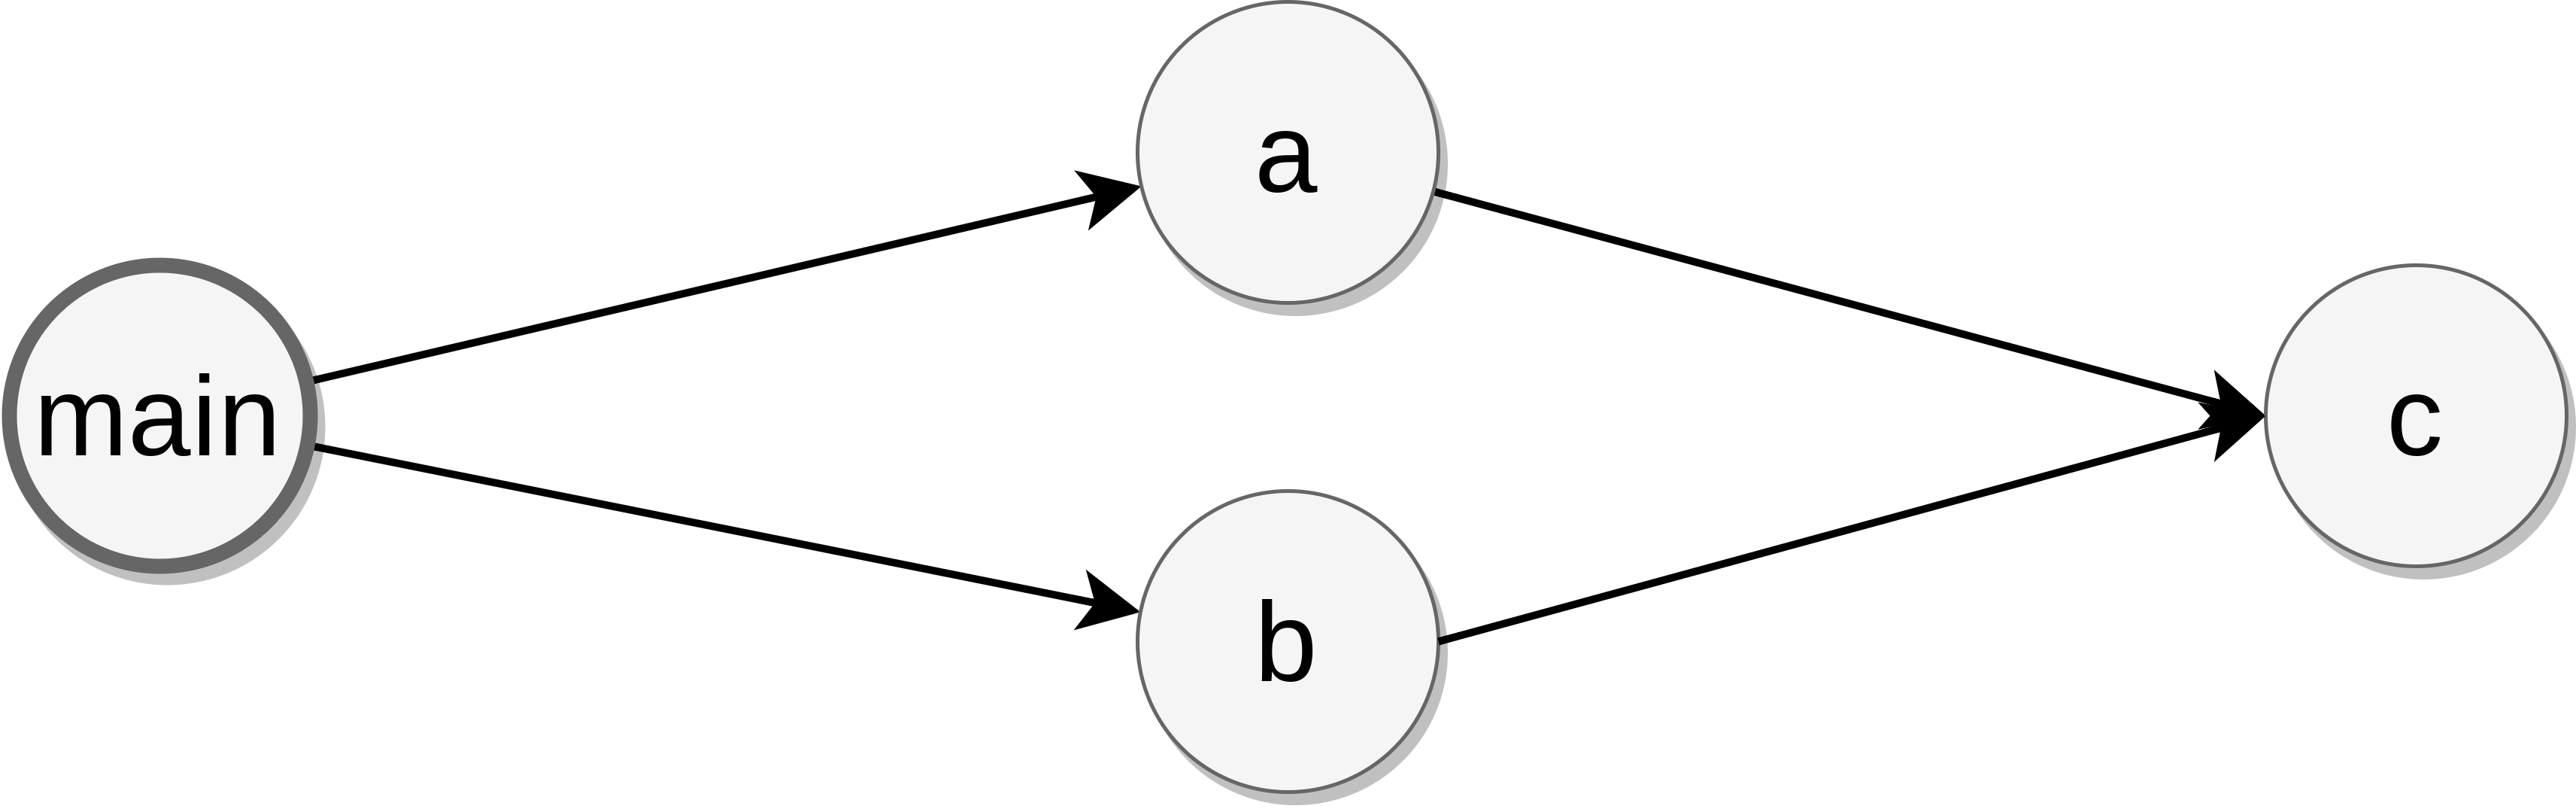
\includegraphics[width=0.8\textwidth]{../images/dependency-tree-Parallel.png}
      \end{center}
    \end{column}
  \end{columns}
\end{frame}

\begin{frame}[fragile]
  \frametitle{PDDL Problem - 1}

  \begin{lstlisting}[style=pddlStyle,basicstyle=\ttfamily\fontsize{10pt}{10pt}\selectfont]
    (:init
      (executed_instruction id0)

      (assignment_id assignmentA id1)
      (assignment_id assignmentB id2)
      (operation_id sumAB id3)
      (assignment_id assignmentC id4)
      
      (dependency_tree id0 id1)
      (dependency_tree id0 id2)
      (dependency_tree id1 id3)
      (dependency_tree id2 id3)
      (dependency_tree id3 id4)
    )

    (:goal (and
      (executed_assignment assignmentA)
      (executed_assignment assignmentB)
      (executed_binary_operation assignmentA assignmentB sumAB assignmentC)
      (executed_assignment assignmentC)
    ))
  \end{lstlisting}
\end{frame}

\begin{frame}[fragile]
  \frametitle{PDDL Problem - 1}

  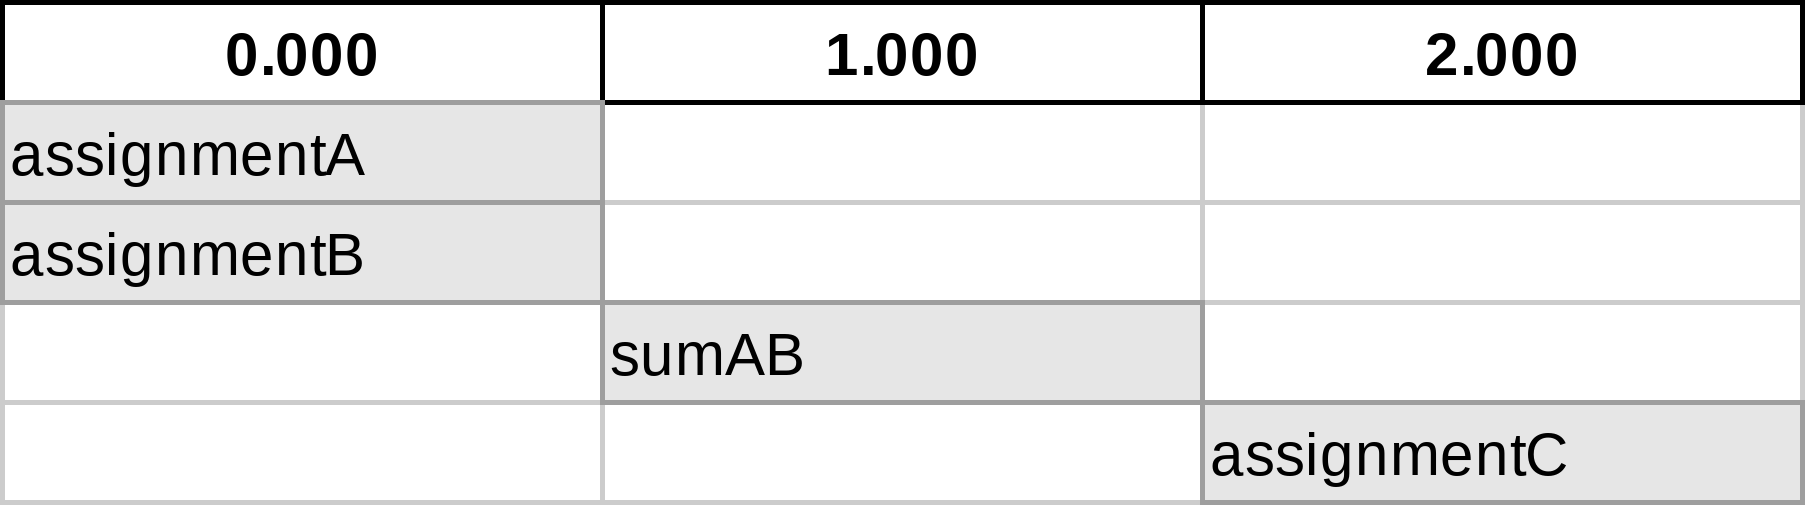
\includegraphics[width=1\textwidth]{../images/parallel-tasks-Parallel.png}
\end{frame}

\begin{frame}[fragile]
  \frametitle{PDDL Problem - 2}

  \begin{columns}
    \begin{column}{0.35\textwidth}
      \begin{lstlisting}[style=cppStyle]
        int main()
        {
          int a = 3;
          int b = a + 1;
          int c = a + b;
          return 0;
        }
      \end{lstlisting}
    \end{column}
    \begin{column}{0.65\textwidth}
      \begin{center}
        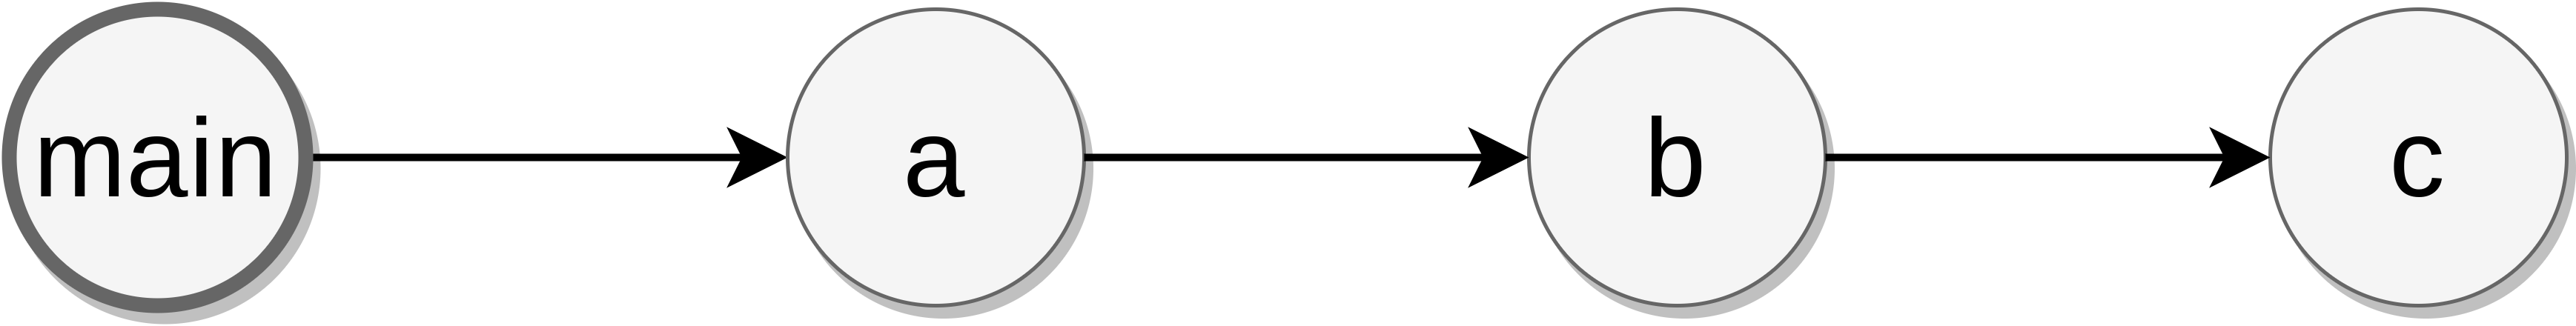
\includegraphics[width=0.8\textwidth]{../images/dependency-tree-NotParallel.png}
      \end{center}
    \end{column}
  \end{columns}
\end{frame}

\begin{frame}[fragile]
  \frametitle{PDDL Problem - 2}

  \begin{lstlisting}[style=pddlStyle,basicstyle=\ttfamily\fontsize{10pt}{10pt}\selectfont]
    (:init
      (executed_instruction id0)

      (assignment_id assignmentA id1)
      (assignment_id assignmentB id2)
      (operation_id sumAB id3)
      (assignment_id assignmentC id4)
      
      (dependency_tree id0 id1)
      (dependency_tree id1 id2)
      (dependency_tree id1 id3)
      (dependency_tree id2 id3)
      (dependency_tree id3 id4)
    )

    (:goal (and
      (executed_assignment assignmentA)
      (executed_assignment assignmentB)
      (executed_binary_operation assignmentA assignmentB sumAB assignmentC)
      (executed_assignment assignmentC)
    ))
  \end{lstlisting}
\end{frame}

\begin{frame}[fragile]
  \frametitle{PDDL Problem - 2}

  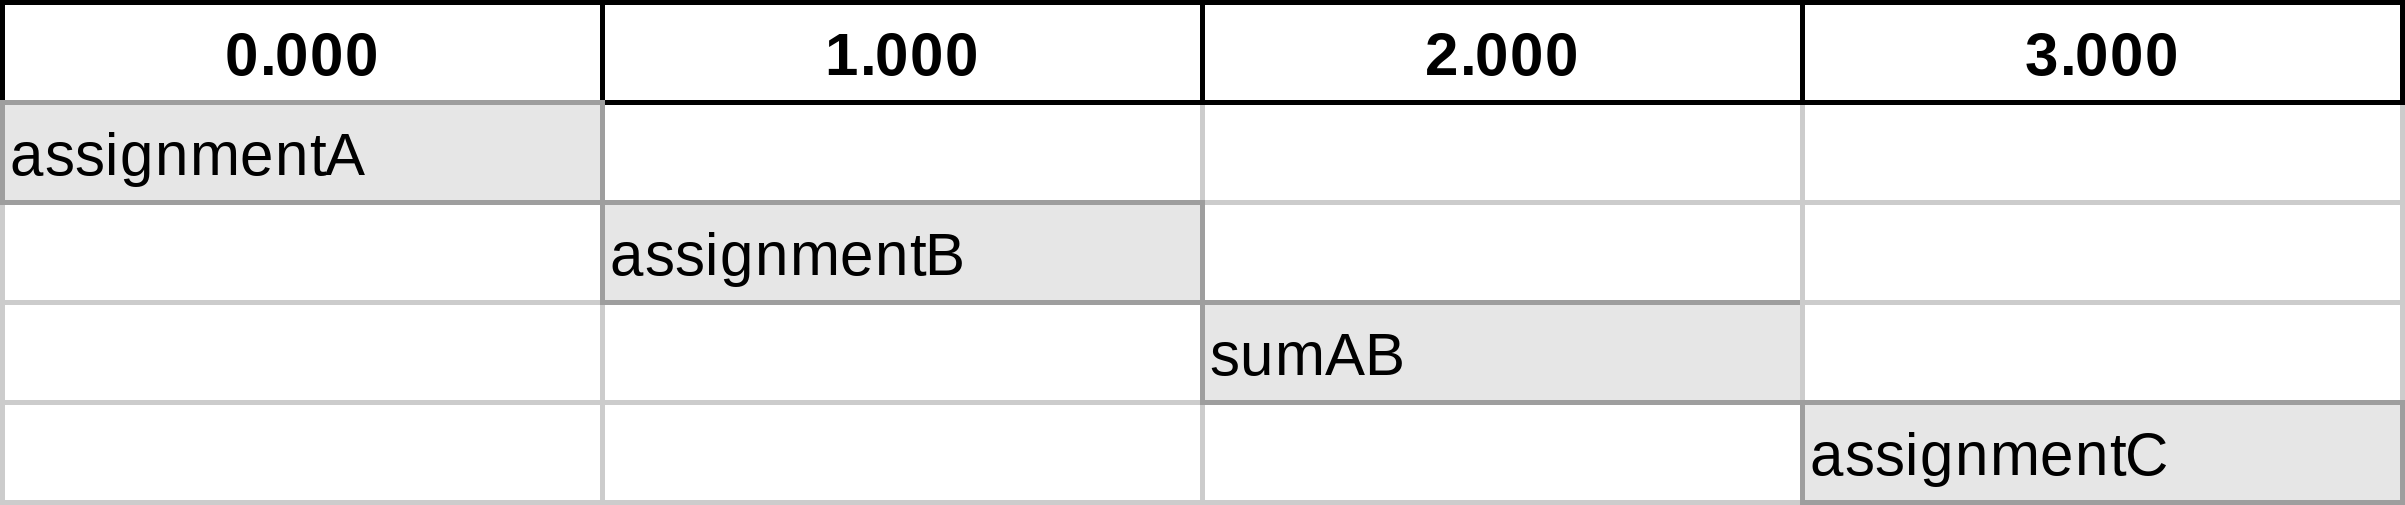
\includegraphics[width=1\textwidth]{../images/parallel-tasks-NotParallel.png}
\end{frame}
%---------------------------------------------------------


%---------------------------------------------------------
\section{Challenges}

\begin{frame}[fragile]
  \frametitle{How to handle \texttt{for} loops?}

  \begin{columns}
    \begin{column}{0.5\textwidth}
      \begin{center}
        \begin{lstlisting}[style=cppStyle,basicstyle=\ttfamily\fontsize{7pt}{7pt}\selectfont]
          int main()
          {
            int s = 0;
            std::vector<int> x = {1, 2, 3};
            for (int i = 0; i < x.size(); i++)
            {
              s += x[i];
            }
            return 0;
          }
        \end{lstlisting}
      \end{center}
    \end{column}
    \begin{column}{0.5\textwidth}
      \begin{center}
        \begin{lstlisting}[style=cppStyle,basicstyle=\ttfamily\fontsize{7pt}{7pt}\selectfont]
          int main()
          {
            int a[3] = {0};
            a[0] = rand();
            for (int i = 1; i < 3; ++i)
            {
              a[i] = a[i - 1] + rand();
            }
            return 0;
          }
        \end{lstlisting}
      \end{center}
    \end{column}
  \end{columns}
\end{frame}

\begin{frame}[fragile]
  \frametitle{PDDL Problem}

  \begin{columns}
    \begin{column}{0.5\textwidth}
      \begin{lstlisting}[style=pddlStyle,basicstyle=\ttfamily\fontsize{7pt}{7pt}\selectfont]
        (:init
          (executed_instruction id0)
    
          (assignment_id assignmentS id1)
          (assignment_id assignmentArray id2)
          (operation_id sum0 id3)
          (assignment_id assignmentS0 id4)
          (operation_id sum1 id5)
          (assignment_id assignmentS1 id6)
          (operation_id sum2 id7)
          (assignment_id assignmentS2 id8)
    
          (dependency_tree id0 id1)
          (dependency_tree id0 id2)
          (dependency_tree id1 id3)
          (dependency_tree id2 id3)
          (dependency_tree id3 id4)
          (dependency_tree id1 id5)
          (dependency_tree id2 id5)
          (dependency_tree id5 id6)
          (dependency_tree id1 id7)
          (dependency_tree id2 id7)
          (dependency_tree id7 id8)
        )
      \end{lstlisting}
    \end{column}
    \begin{column}{0.5\textwidth}
      \begin{lstlisting}[style=pddlStyle,basicstyle=\ttfamily\fontsize{6pt}{6pt}\selectfont]
        (:goal (and
          (executed_assignment assignmentS)
          (executed_assignment assignmentArray)
          (executed_binary_operation assignmentS assignmentArray sum0 assignmentS0)
          (executed_assignment assignmentS0)
          (executed_binary_operation assignmentS assignmentArray sum1 assignmentS1)
          (executed_assignment assignmentS1)
          (executed_binary_operation assignmentS assignmentArray sum2 assignmentS2)
          (executed_assignment assignmentS2)
        ))
      \end{lstlisting}
    \end{column}
  \end{columns}
\end{frame}

\begin{frame}
  \frametitle{stp-2}

  {\scriptsize
    0.000: ( assignment id2 assignmentarray )\\
    0.000: ( assignment id1 assignments )\\
    1.002: ( binary\_operation id3 assignments assignmentarray sum0 assignments0 )\\
    1.002: ( binary\_operation id5 assignments assignmentarray sum1 assignments1 )\\
    2.002: ( binary\_operation id7 assignments assignmentarray sum2 assignments2 )\\
    3.002: ( assignment id4 assignments0 )\\
    3.002: ( assignment id6 assignments1 )\\
    4.002: ( assignment id8 assignments2 )\\
  }
\end{frame}

\begin{frame}
  \frametitle{stp-3}

  {\scriptsize
    0.000: ( assignment id2 assignmentarray )\\
    0.000: ( assignment id1 assignments )\\
    1.002: ( binary\_operation id3 assignments assignmentarray sum0 assignments0 )\\
    1.002: ( binary\_operation id5 assignments assignmentarray sum1 assignments1 )\\
    1.002: ( binary\_operation id7 assignments assignmentarray sum2 assignments2 )\\
    2.002: ( assignment id4 assignments0 )\\
    2.002: ( assignment id6 assignments1 )\\
    3.002: ( assignment id8 assignments2 )\\
  }
\end{frame}
%---------------------------------------------------------


%---------------------------------------------------------
\section{Final Remarks}

\begin{frame}
  \frametitle{Final Remarks}

  \begin{itemize}
    \item It is possible to identify parallel instructions;
  \end{itemize}
  \bigbreak
  \bigbreak
  \begin{itemize}
    \item We need to inform the dependency tree;
    \item How to parse the source code to a PDDL problem?
  \end{itemize}
\end{frame}
%---------------------------------------------------------

\end{document}